\documentclass[journal]{IEEEtran}
\usepackage{graphicx}
\usepackage{subfigure}

\usepackage{hyperref}
\usepackage{multirow}
\usepackage[all]{hypcap} % fix links to figs/tabs

\renewcommand{\arraystretch}{1.1} % make tables more readable

% disable the running header on all pages following the title page
\pagestyle{empty}
%
\begin{document}
% paper title
\title{Applications of GPUs to Online Track Reconstruction in HEP Experiments}
% Author list
\author{S.~Amerio, R.~Ammendola, A.~Biagioni, D.~Bastieri, D.~Benjamin, 
O.~Frezza, S.~Gelain, W.~Ketchum, Y.~K.~Kim, F.~Lo~Cicero, A.~Lonardo, T.~Liu, D.~Lucchesi, P.~S.~Paolucci, S.~Poprocki, D.~Rossetti, F.~Simula, L.~Tosoratto, 
G.~Urso, P.~Vicini, and P.~Wittich
\thanks{Manuscript received November 16, 2012.
This work was supported by the National Science Foundation, the
Department of Energy Office of Science and INFN.}% <-this % stops a space
\thanks{W.~Ketchum and Y.~K.~Kim are with University of Chicago.}%
\thanks{T.~Liu is with Fermi National Accelerator Laboratory.}%
\thanks{S.~Poprocki and P.~Wittich are with Cornell University.}%
\thanks{S.~Amerio is with INFN Padova.}% 
\thanks{R.~Ammendola is with INFN Tor Vergata.}%
\thanks{A.~Biagion, O.~Frezza,  F.~ Lo Cicero, A.~Lonardo, P.~S.~Paolucci, D.~Rossetti,  F.~Simula, L.~Tosoratto and P.~Vicini are with INFN Roma}% 
\thanks{D.~Bastieri, S.~Gelain and D.~Lucchesi are with University of Padova and INFN.}%
\thanks{G.~Urso is with ORMA Software.}%
\thanks{D.~Benjamin is with Duke University.}%
}
% make the title area
\maketitle
% after \maketitle, add the following command to remove the header on the title page
\thispagestyle{empty}
% abstract usually in passive voice
\begin{abstract}
  One of the most important issues that particle physics experiments
  at hadron colliders have to solve is real-time selection of the most
  interesting events. Typical collision frequencies do not allow all
  events to be written to tape for offline analysis, and in most
  cases, only a small fraction can be saved. The most commonly used
  strategy is based on two or three selection levels, with the low
  level ones usually exploiting dedicated hardware to decide within a
  few to ten microseconds if the event should be kept or not. This
  strict time requirement has made the usage of commercial devices 
  inadequate, but recent improvements to Graphics Processing Units (GPUs)
  have substantially
  changed the conditions. Thanks to their highly parallel,
  multi-threaded, multicore architecture with remarkable computational
  power and high memory bandwidth, these commercial devices may be
  used in scientific applications, among which the 
  event selection system (trigger) in particular may benefit, 
  even at low levels. This paper describes the results of an R\&D
  project to study the performance of GPU technology for
  low latency applications, such as HEP fast tracking trigger
  algorithms.  On two different setups, we measure the latency to
  transfer data to/from the GPU, exploring the timing
  of different I/O technologies on different GPU models. We then
  describe the implementation and the performance of a track fitting
  algorithm which mimics the CDF Silicon Vertex Tracker.  These
  studies provide performance benchmarks to investigate the potential
  and limitations of GPUs for future real-time applications in HEP
  experiments.
\end{abstract}

\section{Introduction}
\IEEEPARstart{R}{eal} time event reconstruction plays a fundamental
role in High Energy Physics (HEP) experiments at hadron colliders.
Reducing the rate of data to be saved on tape from millions to
hundreds of events per second is critical. To increase the purity of
the collected samples, rate reduction has to be coupled with an initial
selection of the most interesting events.  In a typical hadron collider experiment, the
event rate has to be reduced from tens of MHz to a few kHz.  The selection system
(trigger) is usually organized in multiple levels, each capable of
performing a finer selection on more complex physics objects
describing the event. Trigger 
systems usually comprise a first level based on custom hardware,
followed by one or two levels usually based on farms of general
purpose processors.  The possibility of also using commercial devices
at a low trigger level is very appealing: they are subject
to continuous performance improvements driven by the consumer market, are
less expensive than dedicated hardware, and are easier to support.  Among
the commercial devices, Graphic Processing Units (GPUs) are of
particular interest for online selections given their impressive
computing power (the latest NVIDIA~\cite{bib_nvidia} GPU architecture,
Kepler, exceeds Teraflop computing power); moreover, high-level
programming architectures based on C/C++ such as
\textsc{cuda}~\cite{bib_cuda} and \textsc{opencl}~\cite{bib_OpenCL}
make these devices more accessible to the general user.  However, GPUs
are not designed for low-latency response, which is a critical
requirement in a trigger system.

We showed initial studies on GPU performance in low-latency
environments ($\sim$100\,$\mu$s) in a previous
paper~\cite{bib_GPU_TIPP2011}.  In this paper we complement those
studies measuring the timing performance of different GPU cards in
different data I/O environments. The algorithm run on the GPU is a
simplified version of the fast track fitting algorithm of the Silicon
Vertex Tracker (SVT) system at CDF~\cite{bib_SVT1}. It has been implemented
and tested on two commercial GPUs (NVIDIA GTX 285 and GTX 590) and on an
NVIDIA Tesla M2075, optimized for scientific and technical
computing. To transfer data to the GPU, we have compared the
performance of S-LINK~\cite{bib_slink} --- 
used in the second level of the CDF trigger system and which we have prior experience with --- and InfiniBand (IB), a more modern protocol.

The goal of this study is to investigate the strengths and weaknesses of
GPUs when applied in a low latency environment, with particular
emphasis on the data transfer latency to/from the GPU and the
algorithm latency for processing on the GPU in a manner similar to
a typical HEP trigger application.


\section{Experimental setup and data flow}
The studies are performed on two different experimental setups,
equipped with different data transfer links and GPU cards.  In both
setups two PCs are used, one acting as a transmitter (TX) and the other 
as a receiver (RX).  Data are transferred from TX to RX, processed on the GPU, and sent back to the receiver (see
Fig.~\ref{fig_data_flow}).  The latency for a complete loop is measured
on the transmitter using the time stamp counter register.

In this setup, the transmitter can represent the detector, as
the source of the data, or an upstream trigger processor, as
the ultimate sink of the data, while the the receiver is the
trigger system: the time to transfer data to the receiver is thus a
rough estimate of the latency to transfer the data from the detector
front-end to the trigger system.
 
The input data is a set of 32-bit words, each representing a set of
hits from the detector. When the track fitting algorithm is run, the
output data is composed of 32-bit words as well, representing the
results of the fit; when the input data is not processed by the fitting algorithm, the output
data is a copy of the input words.
 
\begin{figure}[!h]
\centering
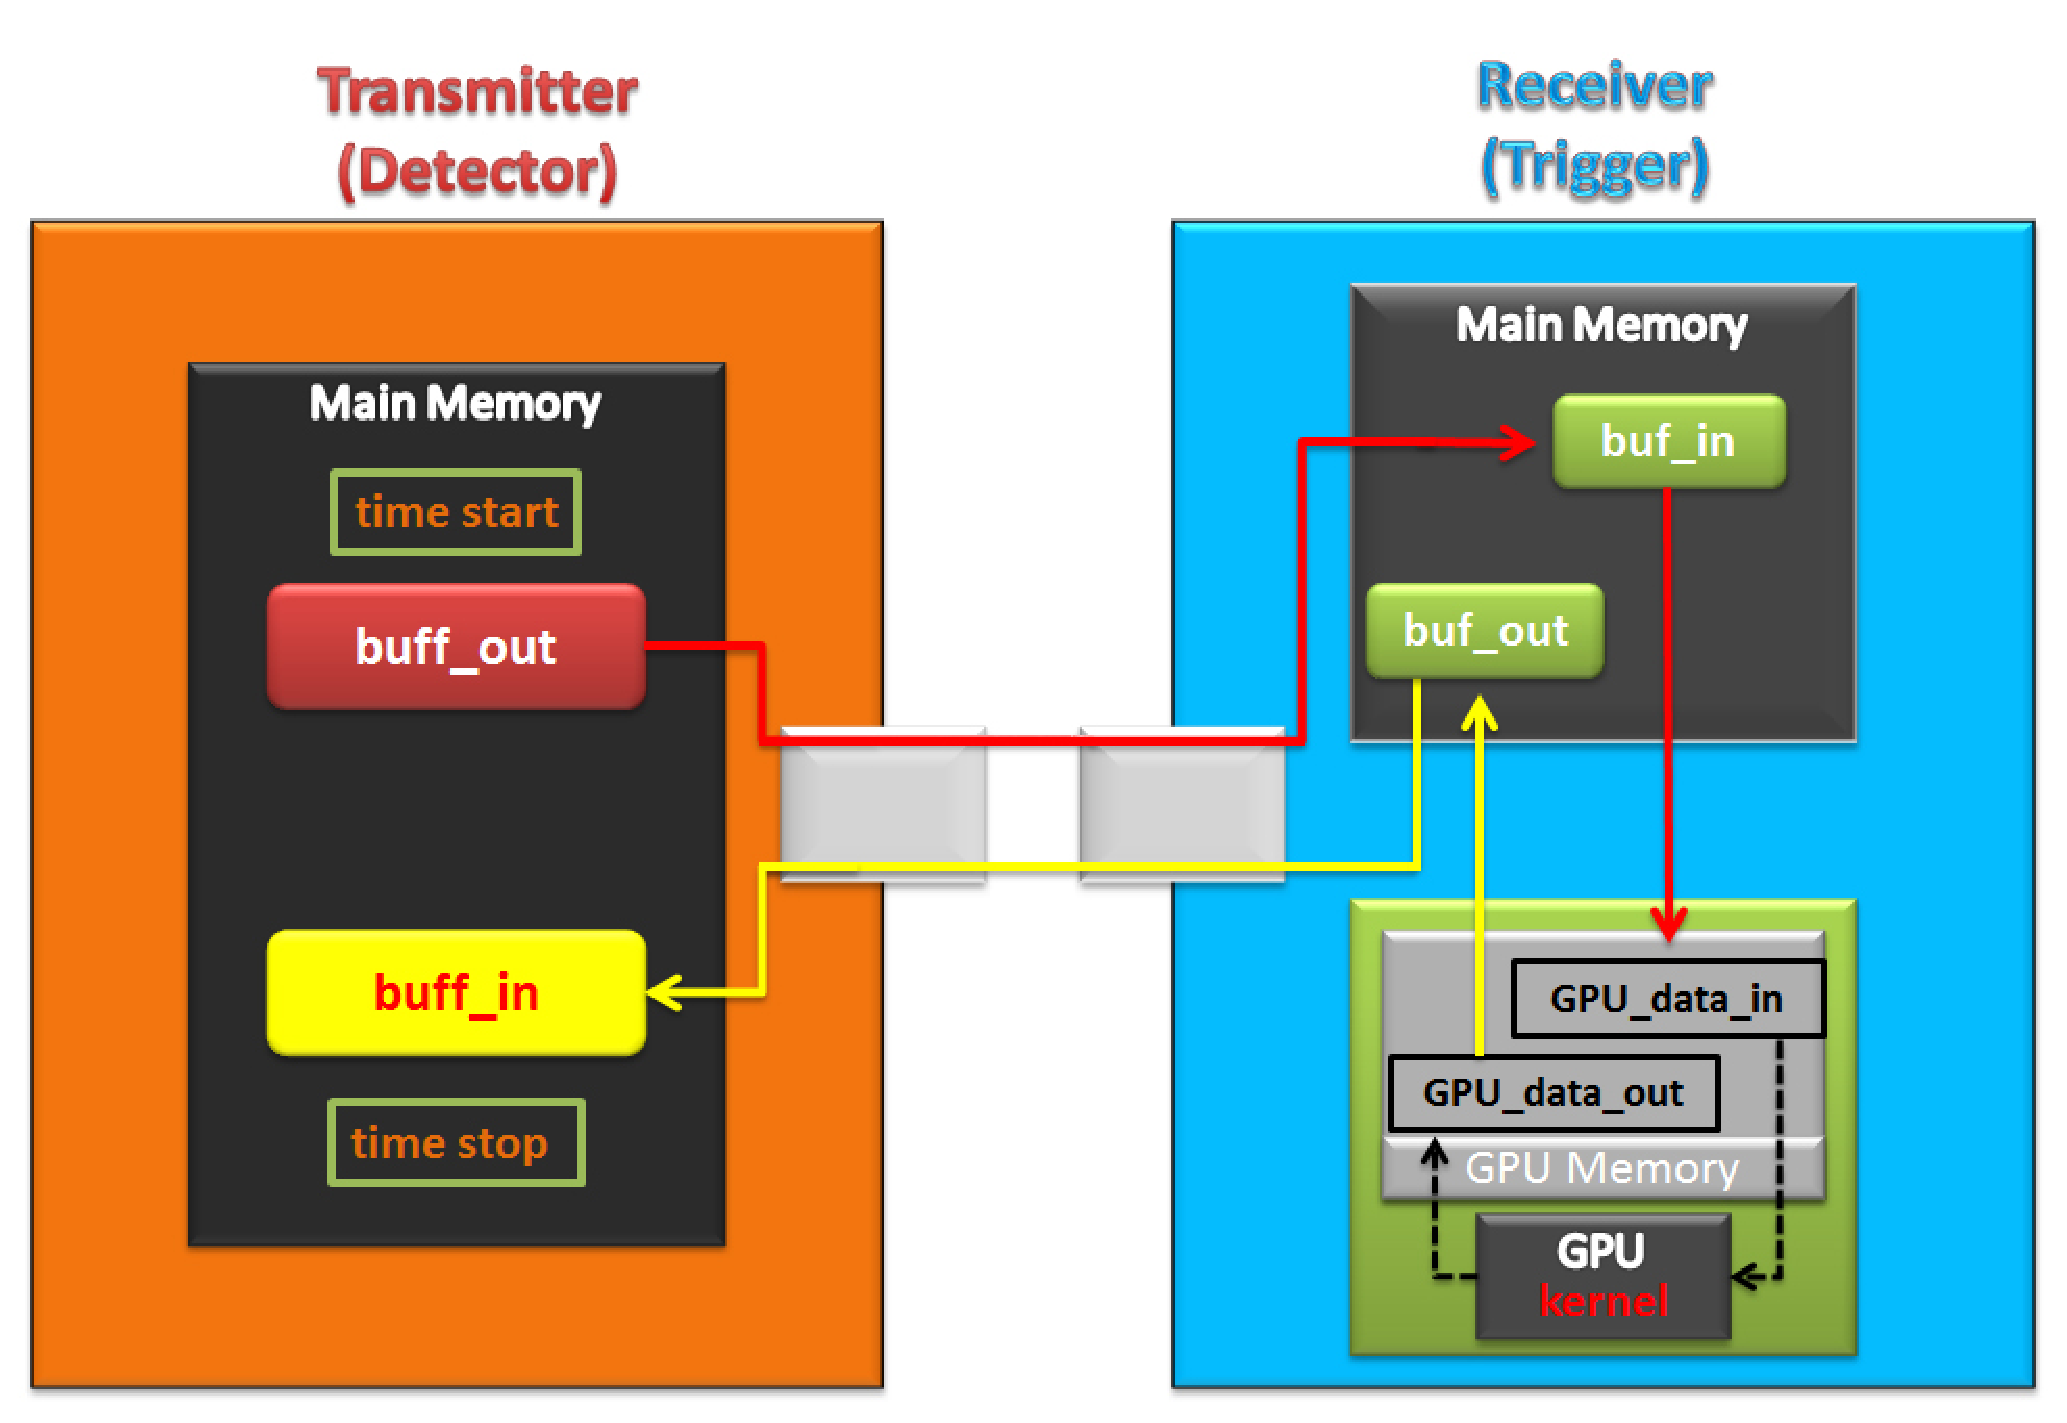
\includegraphics[width=3.5in]{figures/SetUp-general}
\caption{Data flow. Data is sent from the transmitter PC to the
  receiver PC, where it is processed by the GPU before being returned
  to the transmitter PC. The transmitter plays the role of the
  detector as the source of the data and as an upstream trigger
  processor as the data's ultimate sink. The receiver PC plays the
  role of a component in the trigger system. We consider different I/O
  protocols (S-LINK and InfiniBand) and both consumer (GTX) and scientific computing (Tesla) GPUs. }
\label{fig_data_flow}
\end{figure}


\subsection{S-LINK and GTX cards setup}

Both TX and RX PCs are equipped with a CERN FILAR (Four Input Links
for ATLAS Readout)~\cite{bib_filar} and an S32PCI64~\cite{bib_solar}
SOLAR (Single Output Link for ATLAS Readout) PCI interface card for
I/O communication over S-LINK~\cite{bib_slink}.  The TX PC houses two
2.4 GHz AMD Opteron 250 (single core) processors while the RX PC
contains a 3.07 GHz Intel Core i7 CPU 950 (quad core with
hyperthreading) processor.  The RX PC also contains either an NVIDIA GeForce GTX 285 or GTX 590 GPU in a PCIe slot for the GPU computations. A separate GPU handles display operations.


%SILVIA: I propose to remove the following lines as this is repeated 
%before the Data Transfer paragraph.
%The time stamp counter register on the TX PC is used for timing measurements 
%since it is consistent with but has a higher resolution than the high 
%precision Linux timers on this system. Long tails in timing 
%distributions were removed by locking the program to a single CPU core 
%and moving all system interrupts to the remaining CPUs, and running 
%at the highest system scheduler priority, on both PCs. 
%

\subsection{InfiniBand and Tesla cards setup}
The second setup is a computing cluster composed of 12 identical nodes. 
Each node contains a Intel Xeon E6520 2.4 GHz CPU and two Tesla M2075 
GPU cards. The nodes are connected by InfiniBand communication 
links using Connect-X2 Mellanox or Apenet+ adapters. 
Apenet+ is an FPGA-based PCIe board supporting peer-to-peer communication with 
Tesla and Kepler cards~\cite{bib_Apenet}.


\begin{table}[!t]
  \centering
  \begin{tabular}{|l|c|c|c|}
    \hline
    & GTX 285 & GTX 590 & Tesla M2075 \\
    \hline
    \hline
    %Multiprocessors & & & 14 \\
    CUDA cores & 240 & 1024 & 448  \\
    %Peak Single Precision floating point performance (GFlops) & & & 1030 \\
    Memory interface & GDDR3 & GDDR5 & GDDR5 \\
    Memory size (GB) & 1 & 3 & 6  \\
    Memory bandwidth  (GB/s) & 159 & 327 & 150 \\   
    GPUDirect support & No & No & yes \\
    \hline
  \end{tabular}
  \caption{Capabilities of the GPUs used in this study, according to the manufacturer's specifications.}
  \label{tab_GPUcards}
\end{table}
 

\section{Latency measurements}
The data flow can be divided into separate steps, each adding its own 
contribution to the total latency. First, data are transferred from the 
transmitter to the receiver. Once on the receiver, data
are copied to the GPU and then are processed by the GPU. 
%Finally, the output  from the GPU is typically copied back to the receiver PC, and then sent back to the transmitter.

We perform three different sets or measurements:
\begin{enumerate}
\item[A)] Latency for data transfer only:\\
TX $\to$ RX system memory $\to$ TX;
\item[B)] Latency for data transfer and copy to/from the GPU:\\
TX $\to$ RX system memory $\to$ GPU memory $\to$ RX system memory $\to$ TX;
\item[C)] Latency for data transfer, copy to/from the GPU and processing  
in the GPU, where the data flow is the same as above, except a benchmark algorithm is performed in the GPU.
\end{enumerate}

The latency of each round-trip is measured on the transmitter using
the \textsc{rdtsc} time stamp function 
which was found to be consistent with --- but having a higher resolution than --- the high precision Linux timers on our system. 
Each test is repeated 10,000
times and we show the mean and RMS of the repeated measurements. 
To minimize interrupts we use two strategies first developed during the
CDF L2 studies. We use \textsc{cpu affinity} to tie our code to a
single processor, change the scheduler priority of the process to the
highest value (99) and set the scheduling algorithm to
\textsc{sched\_fifo} to ensure that our algorithm does not get removed
from the CPU queue. We also use \textsc{irq affinity} to mask off the
CPU selected above from all interrupts. Fig.~\ref{fig:affinity} shows that 
this setup reduces the long tails in the timing distributions.
\begin{figure}[tbp]
\centering
\includegraphics[width=3.5in]{figures/affinity_32_20121017_irqaffinity}
\caption{Comparison of the timing distributions for default running (solid black)
and for applying CPU \& IRQ affinities and scheduler priority (dashed
red). We see a reduction in the long tails, though some remain. }
\label{fig:affinity}
\end{figure}
However, the timing distributions typically exhibit features such as
multiple humps and long non-Gaussian tails. Preliminarily, we suspect
these features are due to interactions between the CPU and GPU, or
possibly power-saving modes on the GPUs, and further studies are
forthcoming.

\subsection{Data transfer}
Packets of 32-bit words, from a few bytes to 2 MB, are sent from the receiver
to the transmitter and back. No GPU is involved in this measurement.
Due to hardware limitations, the maximum size in input to the S-LINK 
setup is 4 kB.
 
The latency as a function of the packet size is shown in 
Fig.~\ref{fig_DT_SLINK_IB} and in Tab.~\ref{tab_DT}: 
IB shows a linear increase in latency for 
packets up to 2 MB, where 1.4 ms are needed for a complete loop.
A comparison with S-LINK for packets up to 2 kB is presented in the 
inset of the same figure: IB shows lower latencies and a 
smaller slope with increasing packet size. About 13 $\mu$s are needed to 
transfer (round-trip) 4 kB of data. 

\begin{table}[!t]
  \centering
  \begin{tabular}{|r||r|r|}
    \hline
    
    Input  & \multicolumn{2}{|c|}{Data transfer latency ($\mu$s)}  \\     

    (Bytes) & \multicolumn{1}{|c|}{S-LINK}   & \multicolumn{1}{|c|}{IB}\\

    \hline
    \hline
    8    & 12.1 $\pm$ 0.4 & 3.3    $\pm$ 0.3 \\
    %\hline
    32   & 12.6 $\pm$ 0.3 & 3.4    $\pm$ 0.3 \\
    %\hline
    128  & 13.2 $\pm$ 0.4 & 6.1    $\pm$ 0.3 \\
    %\hline
    512  & 16.6 $\pm$ 0.4 & 7.0    $\pm$ 0.2 \\
    %\hline
    1024 & 20.8 $\pm$ 0.2 & 8.3    $\pm$ 0.2 \\
    %\hline
    4096 & 40.3 $\pm$ 0.3 & 13.4   $\pm$ 0.3 \\
    %\hline
    32k  &                & 34.7   $\pm$ 1.8 \\
    %\hline
    65k  &                & 56.0   $\pm$ 1.8 \\
    %\hline
    204k &                & 148.3  $\pm$ 1.1\\
    %\hline
    512k &                & 350.4  $\pm$ 1.8\\
    %\hline
    2M   &                & 1358.1 $\pm$ 1.8\\
    
    \hline
  \end{tabular}
\caption{Data transfer latency. This time measures the round trip 
from the transmitter to the receiver, without interaction to the GPU. }
\label{tab_DT}
\end{table}


\begin{figure}[!t]
\centering
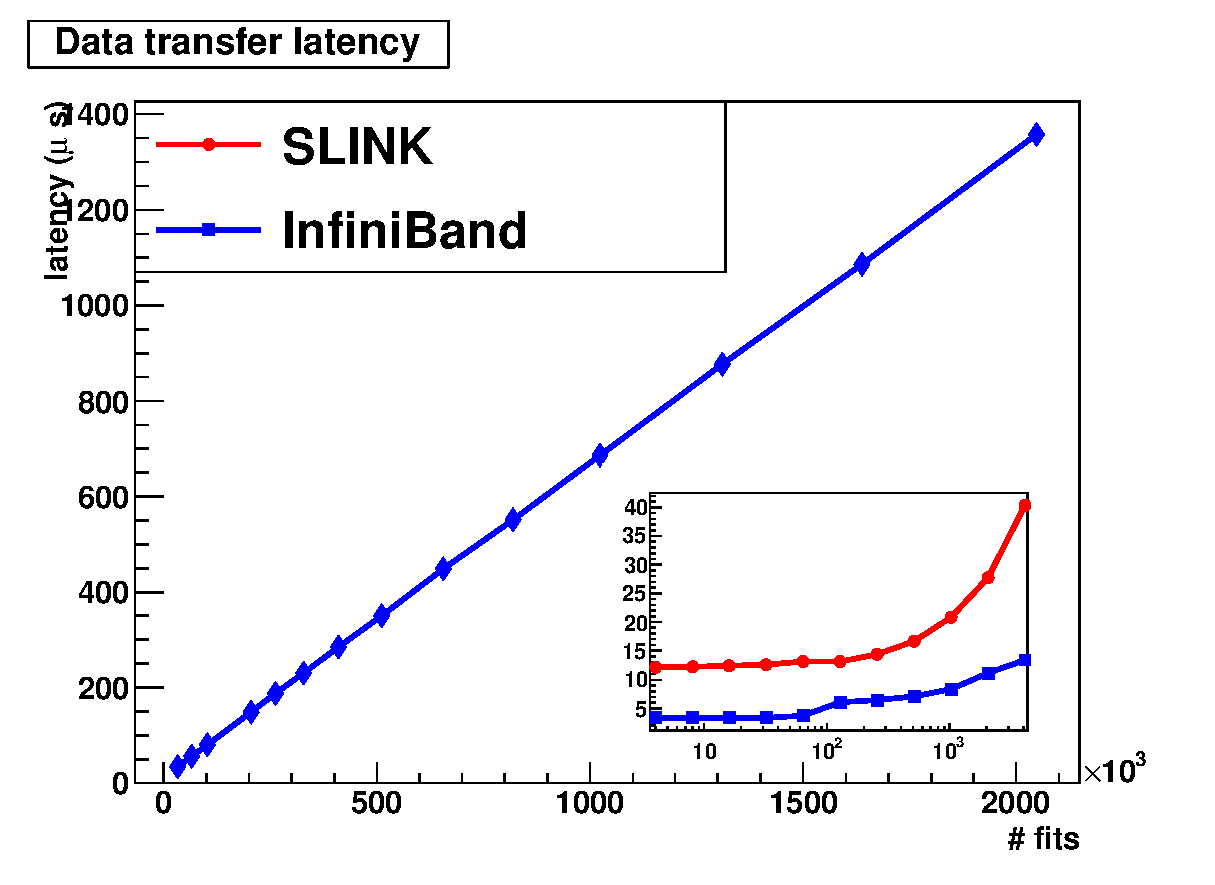
\includegraphics[width=3.5in]{figures/DT_SLINK_IB_inset}
% where an .eps filename suffix will be assumed under latex, 
% and a .pdf suffix will be assumed for pdflatex; or what has been declared
% via \DeclareGraphicsExtensions.
\caption{Data transfer latency as a function of input packets from 32 kB to 
2 MB and for packets from 1 B to 4 kB (inset, logarithmic scale).}
\label{fig_DT_SLINK_IB}
\end{figure}

%\begin{figure}[!h]
%\centering
%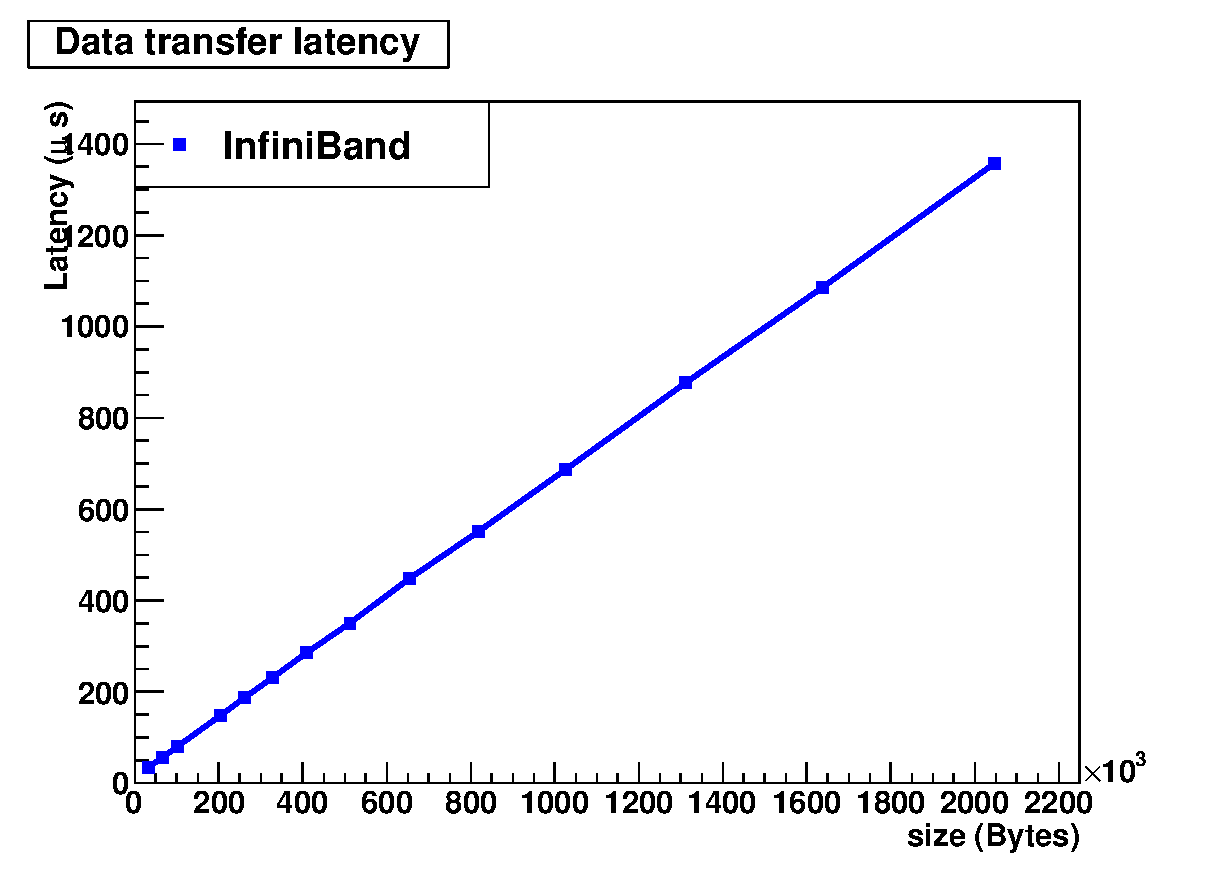
\includegraphics[width=3.5in]{figures/IB_DT_high}
%\caption{Data transfer latency for input packets from 32 kB to 2 MB.}
%\label{fig_DT_IB_HIGH}
%\end{figure}
%
\subsection{Data copy to/from the GPU}

The two experimental setups allow us to test different data transfer 
strategies to the GPU. The standard data transfer strategy is via the 
system memory, where the 
PCIe adapter card and the GPU allocate \emph{separate} buffers on the
system memory for the copy (as shown in Fig.~\ref{fig_standardDT}).
This is inefficient, as the data are copied twice in the 
system memory before being transferred to the GPU/PCIe card. 
Data may also be transferred using Direct Memory Access (DMA, 
GPUDirect\cite{bib_GPUDirect}) to the CPU memory:
the PCIe card and the GPU share the \textit{same} buffer on the CPU memory; as 
a result the data are copied only once in the CPU memory 
(Fig.~\ref{fig_GPUDirectV1}). 
GPUDirect is the standard data transfer mechanism used in the IB-Tesla setup. 
While the GTX GPUs cannot use GPUDirect functionalities, the firmware for S-LINK 
PCI cards allows us to specify an address in system memory where the data is deposited, 
thus achieving a GPUDirect-like setup that avoids an additional copy of the data in system memory.
In the IB-Tesla setup we can test two additional copy 
strategies, which are the results of different levels of 
optimization of the GPUDirect protocol:
\begin{itemize}
\item GPU-Aware MPI, where the copy latency is further reduced
by automatically allocating the buffer on the CPU memory;
\item peer-to-peer (P2P) strategy, when data are transferred 
directly to the GPU, without any  
intermediate copy to the CPU (Fig.~\ref{fig_GPUDirectV2}).
\end{itemize}
%
\begin{figure*}[!t]
\centering
\subfigure[]
{\label{fig_standardDT}
\includegraphics[width=2in]{figures/noGPUDirect}}
\hspace{1mm}
\subfigure[]
{\label{fig_GPUDirectV1}
\includegraphics[width=2in]{figures/GPUDirect}}
\subfigure[]
{\label{fig_GPUDirectV2}
\includegraphics[width=2in]{figures/GPUDirect-APE}}
\caption{Standard data transfer (a), via GPUDirect (b) and via
  GPUDirect with P2P support (c). In (a), two buffers are required in
  the main memory. In GPUDirect (b), one of the main memory buffers is
  eliminated. In GPUDirect with P2P support, data is sent directly
  from the APEnet+ transceiver to the GPU memory.}
\end{figure*}
% No spurious paragraph breaks
As in the previous measurements, packets of varying size are sent to
the receiver, copied from the system memory to the GPU and back, and
finally sent back to the transmitter.  The total round-trip time
(Tab.~\ref{tab_MC}) comprises the data transfer plus copy latency.
Measurements done with the P2P protocol are available only for packets
in the range 32 B -- 4 kB.

For small packet sizes (see Fig.~\ref{fig_DT_MC_SLINK_IB_APE_low}), the 
S-LINK+GTX and IB+Tesla setups show similar performance, about 
30 $\mu$s to transfer 100~B of data. For over 100~B of transferred data,  
the S-LINK latency increases with a much larger slope than IB.
P2P is the best strategy in terms of latency over the whole considered range 
(32 B -- 4 kB).
A comparison between standard GPUDirect and GPU-aware MPI strategy is presented
in Fig.~\ref{fig_DT_MC_GPUDirect_high}. We find that the GPU-Aware MPI 
strategy gives consistent reduction only above 200 kB. 

\begin{table}[!t]
  \centering
  \begin{tabular}{|r||r|r|r|r|}
    \hline
    \multicolumn{1}{|c||}{\multirow{2}{*}{Input}} & \multicolumn{4}{|c|}{Data transfer + copy latency  ($\mu$s)}  \\\cline{2-5}
    \multirow{2}{*}{(Bytes)}
& \multicolumn{2}{|c|}{GPUDirect}
%& \multicolumn{1}{|c|}{GPUDirect}
& \multicolumn{1}{|c|}{GPU-Aware MPI}
& \multicolumn{1}{|c|}{P2P} \\
& \multicolumn{1}{|c|}{(S-LINK)}
& \multicolumn{1}{|c|}{(IB)}
& \multicolumn{1}{|c|}{(IB)}
& \multicolumn{1}{|c|}{(Apenet+)} \\

    \hline
    \hline
     8    & 29.0 $\pm$ 0.3 & 27.1 $\pm$ 2.0   & 27.3 $\pm$ 0.9 &  \\
     %\hline
     32   & 29.3 $\pm$ 0.1 & 27.5 $\pm$ 0.7   & 27.5 $\pm$ 2.4 &  18.1 $\pm$ 1.2 \\
     %\hline                               
     128  & 32.6 $\pm$ 1.0 & 29.6 $\pm$ 0.7   & 28.9 $\pm$ 1.9 &  20.6 $\pm$ 3.0\\
     %\hline                               
     512  & 38.6 $\pm$ 0.9 & 30.8 $\pm$ 0.7   & 31.5 $\pm$ 0.8 &  20.8 $\pm$ 2.4\\
     %\hline                               
     1024 & 46.1 $\pm$ 1.0 & 32.6 $\pm$ 1.7   & 33.5 $\pm$ 2.3 &  21.2 $\pm$ 2.6\\
     %\hline                               
     4096 & 86.3 $\pm$ 0.7 & 39.1 $\pm$ 2.2   & 40.5 $\pm$ 1.1  &  25.6 $\pm$ 3.0\\
     %\hline                               
     32k  &                & 66.4 $\pm$ 2.3   & 84.9 $\pm$ 2.7 &\\
     %\hline                               
     65k  &                & 98.9 $\pm$ 2.1   &  115.4 $\pm$ 2.8 &\\
    %\hline
     204k &                & 230.3 $\pm$ 2.4  &  231.0 $\pm$ 4.1 &\\
     %\hline
     512k &                & 511.6 $\pm$ 3.3  &  413.0 $\pm$ 3.5 &\\
     %\hline
     2M   &                & 1917.8 $\pm$ 6.2 &  1330.5 $\pm$ 4.5 &\\
     
    \hline
  \end{tabular}
\caption{Latency for data transfer plus copy to/from the GPU. The S-LINK measurements here are taken using the GTX 590 GPU, while the IB and Apenet+ measurements use the Tesla M2075 GPU.}
\label{tab_MC}
\end{table}


\begin{figure}[!t]
\centering
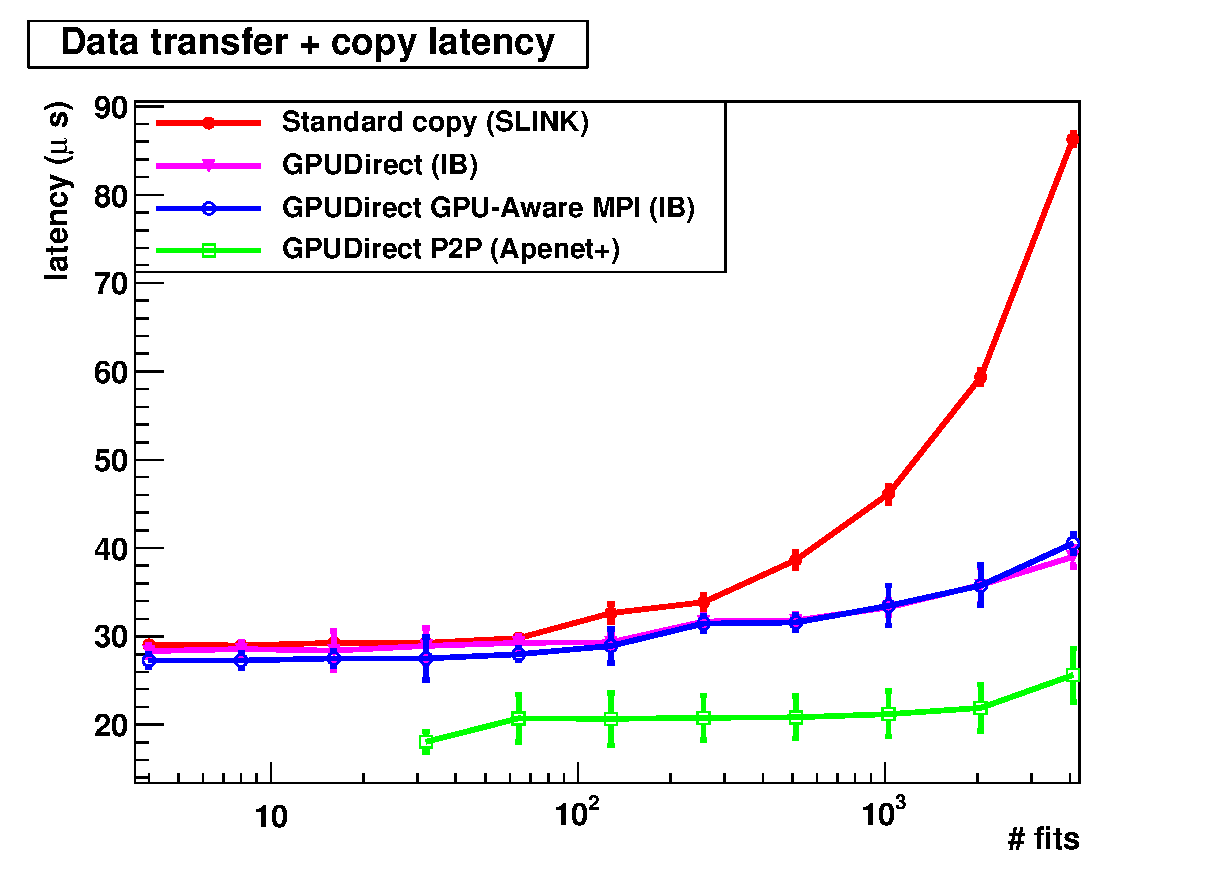
\includegraphics[width=3.5in]{figures/DT_MC_SLINK_IB_APE_low}
\caption{Data transfer plus copy latency for GPUDirect standard, 
GPU-Aware MPI and P2P. Input packet size from 1 B (32 B for Apenet+) to 4 kB.}
\label{fig_DT_MC_SLINK_IB_APE_low}
\end{figure}




\begin{figure}[!t]
\centering
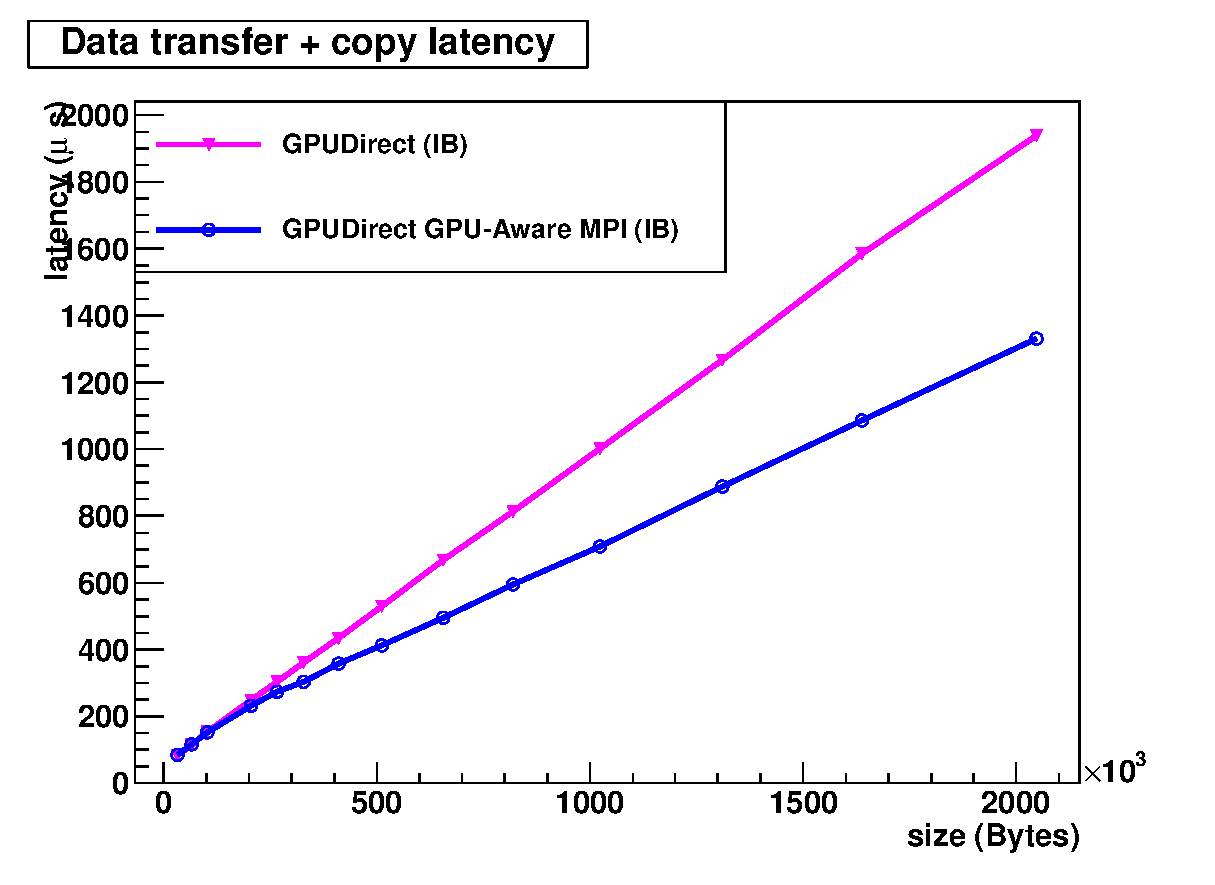
\includegraphics[width=3.5in]{figures/MC_IB_high}
\caption{Data transfer plus copy latency for GPUDirect standard 
 and GPU-Aware MPI up to 2 MB.}
\label{fig_DT_MC_GPUDirect_high}
\end{figure}



\subsection{Data processing on the GPU}

Many tasks performed by trigger systems may benefit from the 
parallelization available in a GPU (e.g. jet clustering and track finding). 
For this study, we choose as a benchmark a simplified fast track-fitting
algorithm which was used in CDF's Silicon Vertex Trigger 
(SVT)~\cite{bib_SVT1}~\cite{bib_SVT2}.
This algorithm uses a linearized approximation to track-fitting as 
implemented in hardware (described in greater detail in~\cite{bib_SVT3}). 
With the SVT approach, the determination of the track parameters 
($p_i$) is reduced to a simple scalar product:
\[
p_i = \vec{f_i} \cdot \vec{x_i} + q_i,
\]
where $\vec{x_i}$ are input silicon hits, and $\vec{f_i}$ and $q_i$ are 
pre-defined constant sets. For each set of hits, the algorithm
computes the impact parameter $d_0$, the azimuthal angle $\phi$, 
the transverse momentum $p_\mathrm{T}$ , and the $\chi^2$ of the
fitted track by using simple operations such as memory lookup and 
integer addition and multiplication. In
our testing of the track-fitting algorithm, each word in input is treated to
represent a set of silicon hits. While the track-fitting algorithm 
itself is simple, it must be performed on
many combinations of hits in a given event, especially in high-occupancy 
environments. This makes it a good 
benchmark for testing performance of a GPU, using massive parallelization at low latencies.

In Figs.~\ref{fig_DT_MC_TF_SLINK} and \ref{fig_DT_MC_TF_IB_low}
and Tabs.~\ref{tab_TF_SLINK} and \ref{tab_TF_IB},
the total latency for data transfer, 
copy to the GPU, and processing in the GPU is shown. For comparison, 
 the distributions for data transfer and data transfer plus copy are 
superimposed. 

\begin{table}[!t]
  \centering
  \begin{tabular}{|r||r|r|r|}
    \hline

    \multirow{2}{*}{Input (Bytes)} & \multicolumn{3}{|c|}{ Latency  ($\mu$s)}  \\     
    
                                   & \multicolumn{1}{|c|}{Data transfer}
                                   & \multicolumn{1}{|c|}{+ copy}
                                   & \multicolumn{1}{|c|}{+ calculations} \\

    \hline
    \hline
    128 & 13.2 $\pm$ 0.4 & 32.6 $\pm$ 1.0 & 39.5 $\pm$ 1.4 \\ 
    256 & 14.4 $\pm$ 0.4 & 33.9 $\pm$ 0.8 & 41.6 $\pm$ 1.5 \\ 
    512 & 16.6 $\pm$ 0.4 & 38.6 $\pm$ 0.9 & 46.8 $\pm$ 1.4 \\ 
    1024 & 20.9 $\pm$ 0.2 & 46.1 $\pm$ 1.0 & 53.9 $\pm$ 1.4 \\ 
    2048 & 27.7 $\pm$ 0.3 & 59.4 $\pm$ 0.8 & 67.1 $\pm$ 1.2 \\ 
    4096 & 40.3 $\pm$ 0.2 & 86.3 $\pm$ 0.7 & 93.9 $\pm$ 1.0 \\      
    \hline
  \end{tabular}
\caption{Data transfer + copy + calculation latency (S-LINK + GTX 590).}
\label{tab_TF_SLINK}
\end{table}

\begin{table}[!t]
  \centering
  \begin{tabular}{|r||r|r|r|}
    \hline

    \multirow{2}{*}{Input (Bytes)} & \multicolumn{3}{|c|}{ Latency  ($\mu$s)}  \\     
    
                                   & \multicolumn{1}{|c|}{Data transfer}
                                   & \multicolumn{1}{|c|}{+ copy}
                                   & \multicolumn{1}{|c|}{+ calculations} \\

    \hline
    \hline
     8    & 3.3 $\pm$ 0.3   & 27.1 $\pm$ 2.0 & 33.3 $\pm$ 2.1\\
     %\hline
     32   & 3.4 $\pm$ 0.3   & 27.5 $\pm$ 0.7 & 33.2 $\pm$ 2.0\\
     %\hline
     128  & 6.1 $\pm$ 0.3  & 29.6 $\pm$ 0.7 & 35.7 $\pm$ 2.0\\
     %\hline
     512  & 7.0 $\pm$ 0.2  & 30.8 $\pm$ 0.7 & 36.5 $\pm$ 2.6\\
     %\hline
     1024 & 8.3 $\pm$ 0.2  & 32.6 $\pm$ 1.7 & 37.9 $\pm$ 2.7\\
     %\hline
     4096 &  13.4 $\pm$ 0.3 &  39.1 $\pm$ 2.2 & 45.8 $\pm$ 2.1\\
%     %\hline
%     32k  &  34.7 $\pm$ 1.8 &   66.4 $\pm$ 2.3 & 75.4 $\pm$ 3.9\\
%     %\hline
%     262k & 187.6 $\pm$ 1.1 & 280.2 $\pm$ 2.5 & 298.1 $\pm$ 2.7\\
%     %\hline
%     512k & 350.4 $\pm$ 1.8 & 511.7 $\pm$ 3.3 &   534.2 $\pm$ 4.4\\
%     %\hline
%     2M   &  1358.1 $\pm$ 1.8 & 1917.8 $\pm$ 6.2 & 2001.8 $\pm$ 6.8\\
%     
    \hline
  \end{tabular}
\caption{Data transfer + copy + calculation latency (IB + Tesla M2075).}
\label{tab_TF_IB}
\end{table}

\begin{figure}[!t]
  \centering
  \subfigure[]
{\label{fig_DT_MC_TF_SLINK}
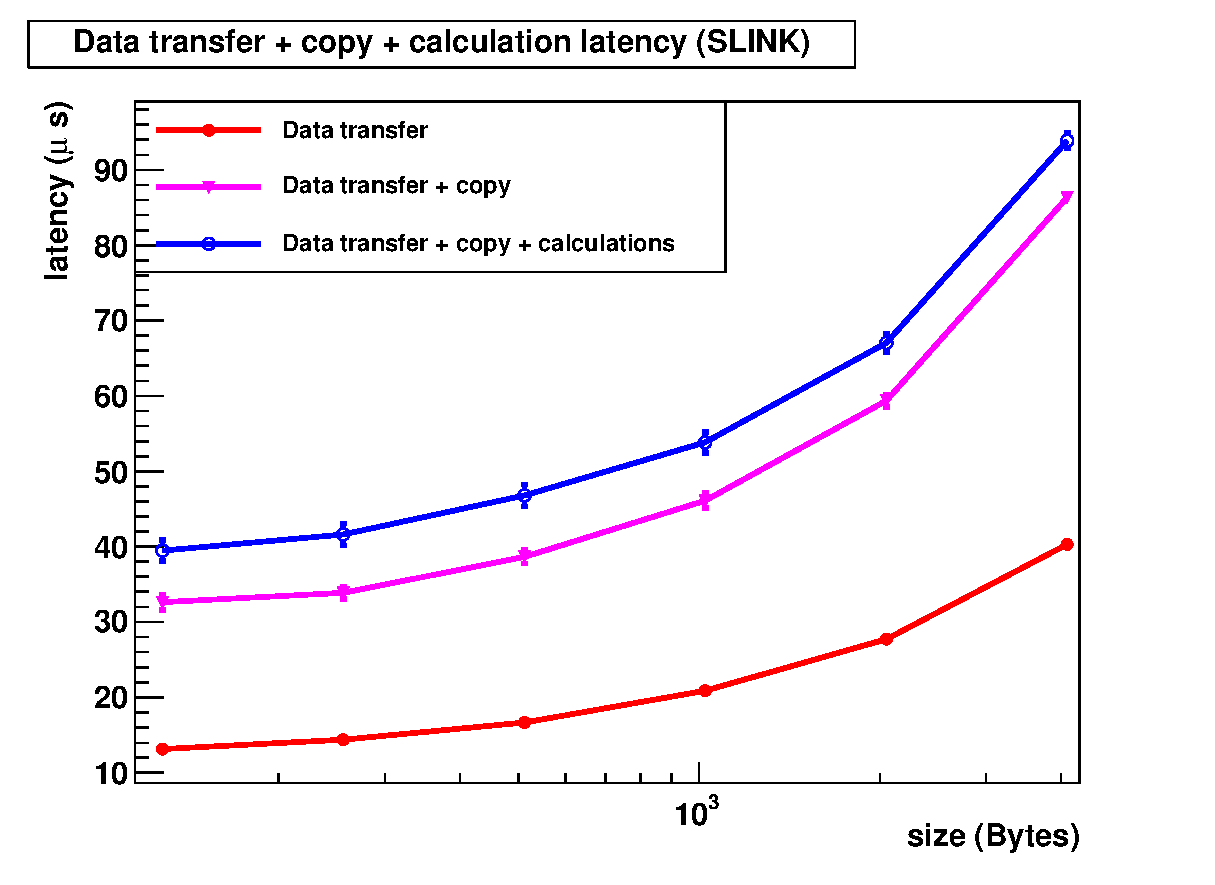
\includegraphics[width=3.5in]{figures/DT_MC_TF_SLINK}}
\hspace{1mm}
\subfigure[]
{\label{fig_DT_MC_TF_IB_low}
 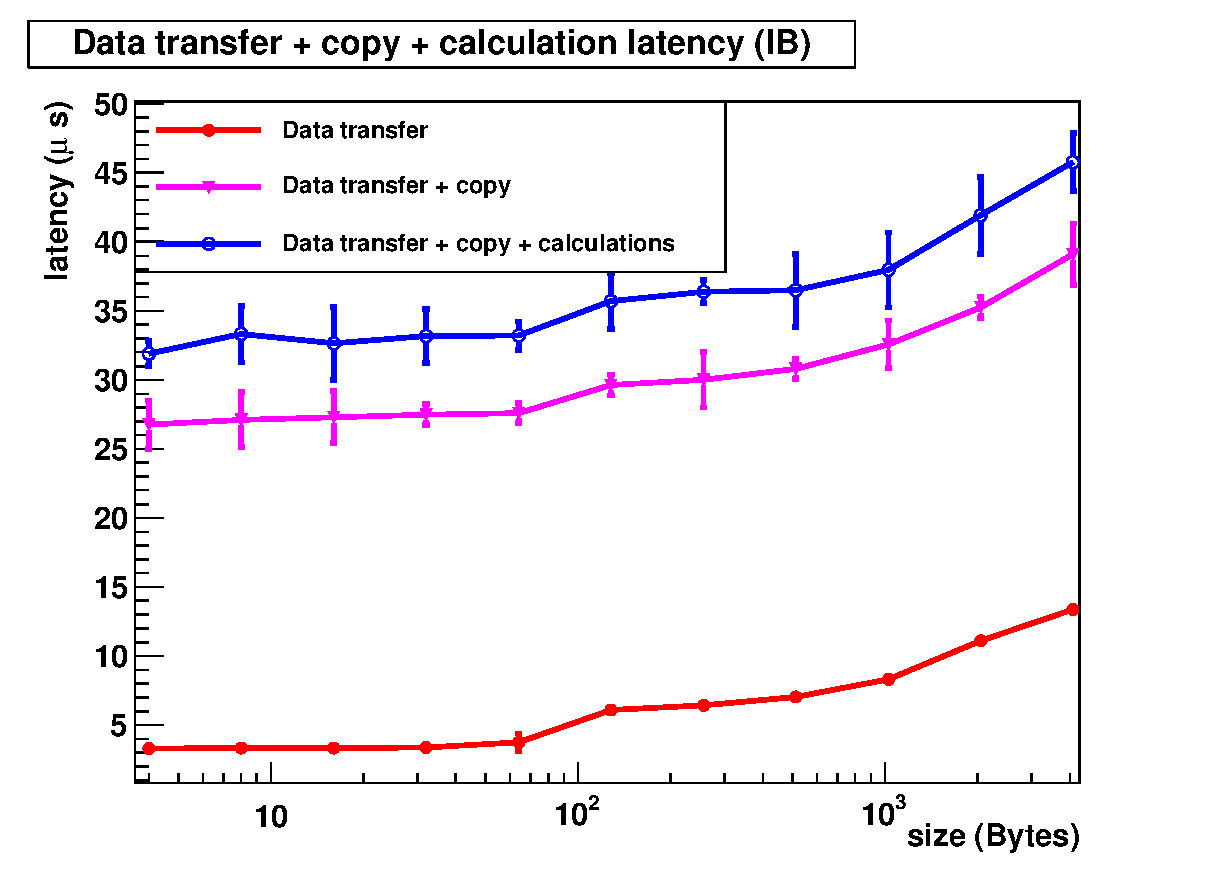
\includegraphics[width=3.5in]{figures/DT_MC_TF_IB_low}}
\caption{Total latency for data tranfer, copy to/from the GPU and data 
processing on the GPU, for S-LINK and GTX 590 card (a) and for IB and Tesla M2075 card (b). Note the $y$ axis goes up to 90 $\mu$s in (a) and 50 $\mu$s in (b).} 
\end{figure}


%\begin{figure}[!h]
%  \centering
%  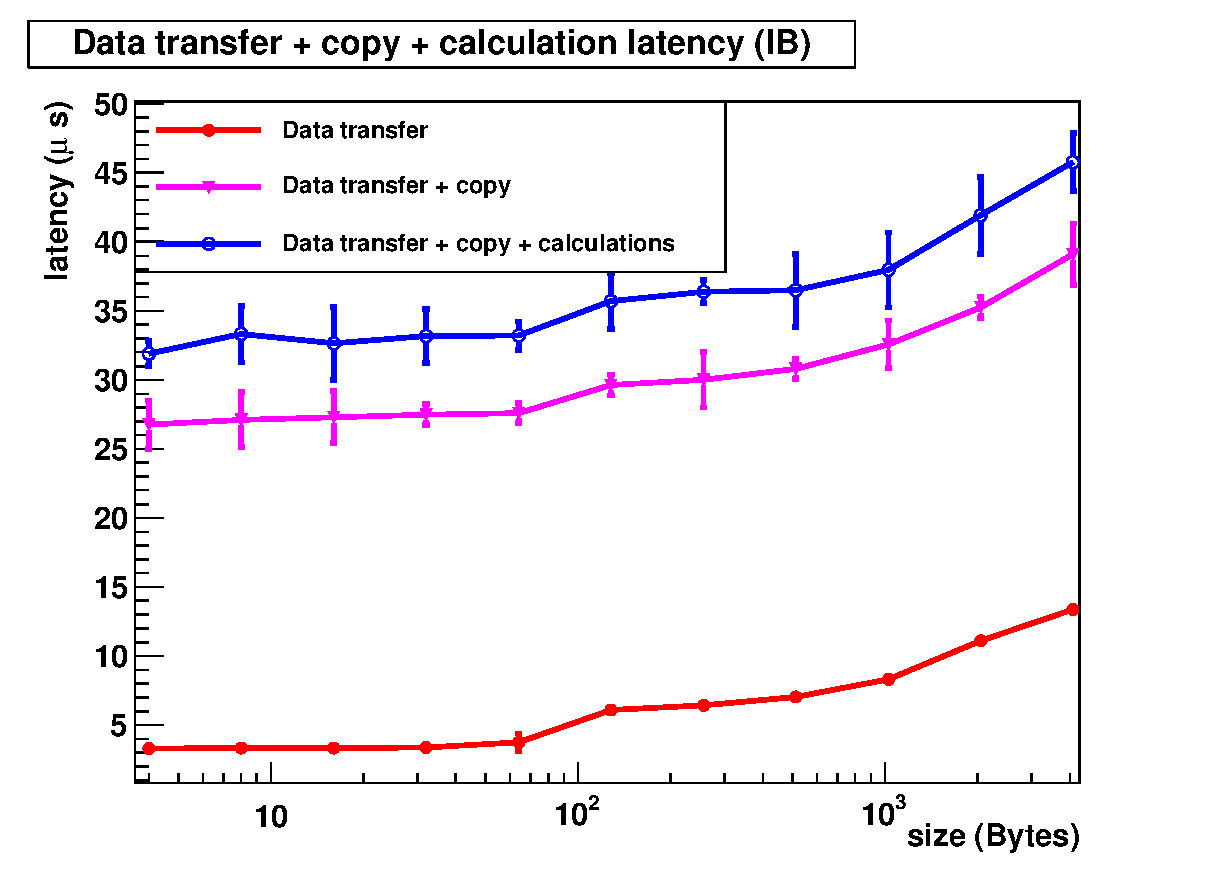
\includegraphics[width=3.5in]{figures/DT_MC_TF_IB_low}
%  \caption{Total latency for data tranfer, copy to/from the GPU and data 
%processing on the GPU, for IB and Tesla card.}
%  \label{fig_DT_MC_TF_IB_low}
%\end{figure}
% 
Adding the track fitting algorithm on the GPU, the latency increases of
about 8~$\mu$s for the GTX 590 card and 6 $\mu$s for the Tesla. 
The two cards have similar performance in terms of calculation latency. 
The increase in the total latency is fixed as a function of 
the input data (\textit{i.e.}, the number of calculations since each input 
word is a track to be fitted), due to the parallel nature of the 
calculations inside the GPU.

This is visible also in Fig.~\ref{fig_TF_SLINK_IB_fixedSize}, where the total 
latency is measured for fixed input (2 kB) and output (256 kB) size, and 
only the number of fits is varied, from 32 to 16,384. The latency 
distribution is flat up to 1,000 fits and shows a slight slope 
for larger numbers of fits. The slope is largest for the GTX 285, as 
expected, due to it having the fewest number of CUDA cores.
In this plot the latency is dominated by the time needed to transfer 
the output back to the transmitter.
Moreover, each point is the mean 
over 10 different runs, and the error is the relative error on the mean: 
the smaller this error, the smaller the run-by-run spread --- a highly 
desirable feature in any real-time event selection system. In both experimental
setups we find that the run-by-run spread is in the range of 1.5 -- 3 $\mu$s. 

\begin{figure}[!t]
  \centering
  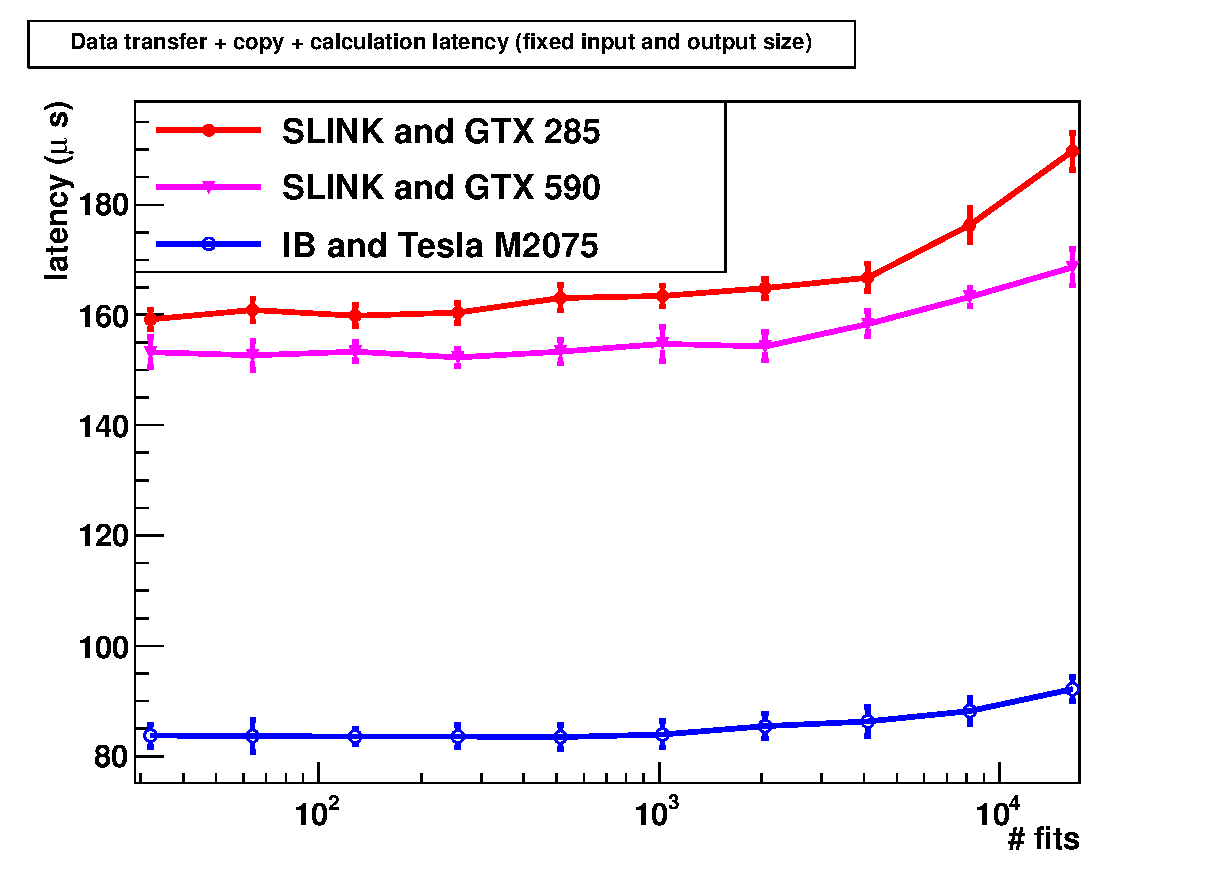
\includegraphics[width=3.5in]{figures/TF_SLINK_IB_fixedSize}
  \caption{Total latency (data transfer, copy and track fitting algorithm) for the three different GPU cards used in this study.}
  \label{fig_TF_SLINK_IB_fixedSize}
\end{figure}


Figure~\ref{fig_TF_SLINK_IB_fixedSize_CPUvsGPU}
shows the latency for the same SVT-like track fitting
algorithm run on the CPU of the experimental setup, compared to the
performance on the GPU.  We stress that the algorithm is run on a
single core of the CPU and it is not optimized for the CPU.  The data
transfer time has been subtracted, so the latency is due only to the
calculations and to the copy to/from the GPU.  The GPU has much better
performance for a large number of fits, while it is surpassed by the
CPU for small number of calculations, as would be expected due to the
excellent multi-threaded processing of GPUs.


\begin{figure}[!h]
  \centering
  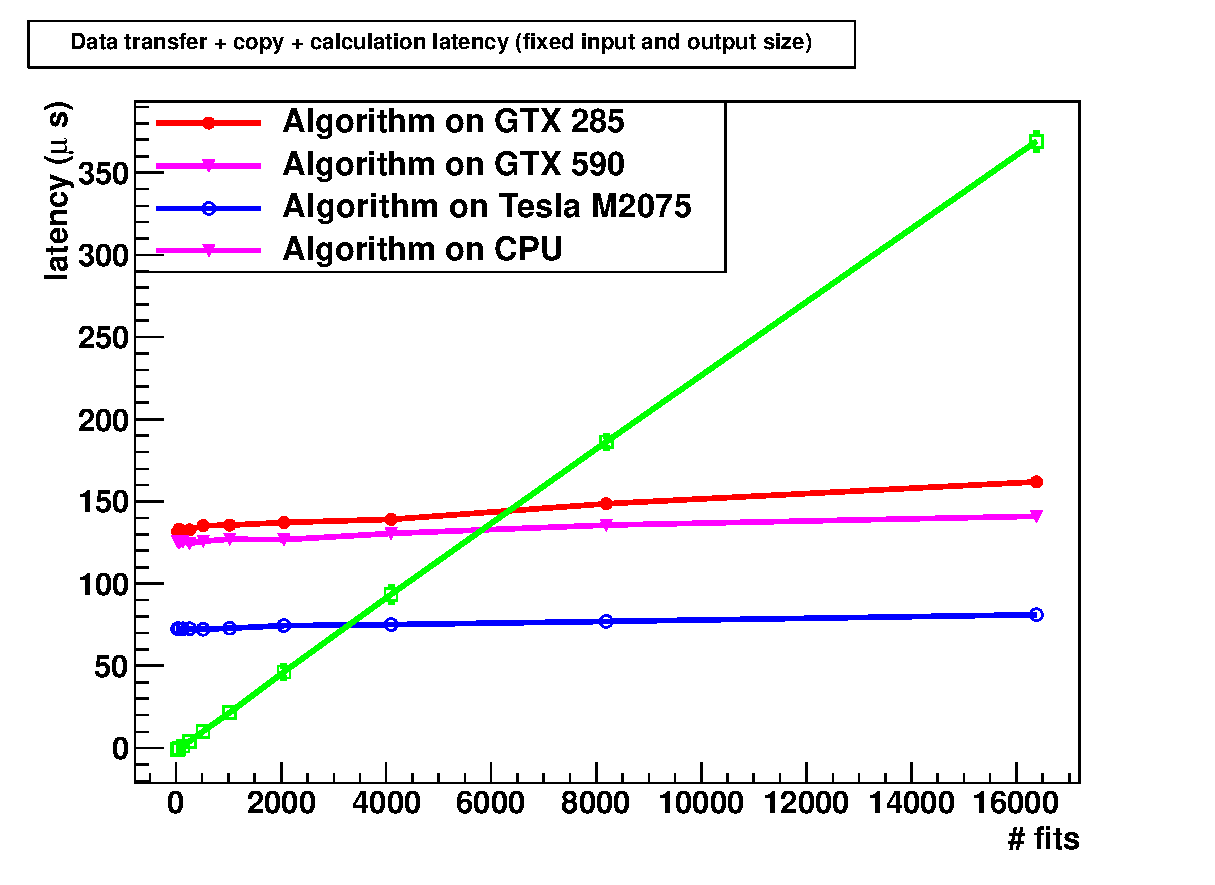
\includegraphics[width=3.5in]{figures/TF_SLINK_IB_fixedSize_CPUvsGPU_noDT}
  \caption{Comparison of the algorithm latency on the different GPUs 
to the total latency for the same algorithm run on the CPU (IB 
experimental setup only), as a function of the number of threads.  As would
be expected, the GPU performs better for a large number of fits.}
  \label{fig_TF_SLINK_IB_fixedSize_CPUvsGPU}
\end{figure}

%\begin{figure}[!h]
%  \centering
%  \subfigure[]
%{\label{fig_TF_SLINK_fixedSize_CPUvsGPU}
%\includegraphics[width=3.5in]{figures/TF_SLINK_fixedSize_CPUvsGPU_noDT}}
%\hspace{1mm}
%\subfigure[]
%{\label{fig_TF_IB_fixedSize_CPUvsGPU}
% \includegraphics[width=3.5in]{figures/TF_IB_fixedSize_CPUvsGPU_noDT}}
%\caption{Comparison of the algorithm latency on GPU to the total latency 
%for the same algorithm run on the CPU of the S-LINK (a) and IB (b) 
%experimental setups, as a function of the number of threads.  As would
%be expected, the GPU performs better for a large number of fits. } 
%\end{figure}
%
\subsection{Conclusions}

Following up on initial studies of GPUs to low-latency applications in HEP experiments, 
we have performed additional benchmark measurements for a variety of GPUs and data transfer 
strategies. We see improvements in latency for the more modern InfiniBand communication link 
protocol, compared to the S-LINK protocol. More importantly, we see smaller latencies for the time
it takes to copy memory into the GPU when using some of NVIDIA's GPUDirect utilities. Using GPU-Aware MPI
leads to a decrease in that memory transfer time for large data sizes, while using peer-to-peer communication
strategies shows a strong boost to performance for even small data sizes. As shown in 
Tabs.~\ref{tab_TF_SLINK} and \ref{tab_TF_IB}, the time to copy memory into and out of the GPU represents a significant overhead 
for the total latency. These and other strategies for improving the memory transfer speed, along with a smarter implementation of 
algorithms which reduces the amount of memory transfers, will make GPUs more viable for low-latency applications.

We have also conducted a comparison of different GPUs, showing latency 
measurements for two commercial GPUs (the GTX 285 and GTX 590 from NVIDIA) 
and a GPU optimized for scientific and technical computing (the Tesla M2075, 
also manufactured by NVIDIA). The performance in the InfiniBand+Tesla setup is 
better, but much of this is from the aforementioned memory transfer improvements.
When looking only at the additional latency when performing the track-fitting algorithm, 
the performance of the GTX and Tesla class GPUs are comparable in the region we explored.

Finally, we performed tests while holding the input and output data sizes fixed, only varying the number of 
calculation threads on the GPU. While there is some increase in latency with an increase in the number of
calculation threads, that increase is rather small, especially compared to running the same number of 
calculations on a single CPU thread. If the overhead times can be controlled or even further reduced, GPUs 
may offer a flexible and cost-effective way to achieving a high level of parallelization in applications that demand low latency.



%%%% IEEE wants placement as !t
%\begin{figure}[!t]
%\centering
%%\includegraphics[width=3.5in]{myFigure}
%% where an .eps filename suffix will be assumed under latex, 
%% and a .pdf suffix will be assumed for pdflatex; or what has been declared
%% via \DeclareGraphicsExtensions.
%\caption{Daily abstract submission rate of the 2012 NSS-MIC. }
%\label{fig_sim}
%\end{figure}
%

% use section* for acknowledgement
\section*{Acknowledgment}
The authors would like to thank the Fermilab staff and the FTK group at the 
University of Chicago for their support. This work was supported by the
U.S. Department of Energy and National Science Foundation and the Italian
Istituto Nazionale di Fisica Nucleare. 

\begin{thebibliography}{99}
\bibitem{bib_nvidia} \url{http://www.nvidia.com}
\bibitem{bib_cuda}\url{http://www.nvidia.com/object/cuda_home_new.html}
\bibitem{bib_OpenCL}\url{http://www.khronos.org/opencl/}
\bibitem{bib_GPU_TIPP2011} W.~Ketchum \textit{et al.}, \emph{Performance Study of GPUs in Real-Time Trigger Applications for HEP Experiments},  Physics Procedia, Volume 37, 2012, 1965-1972.
\bibitem{bib_filar} W. Iwanski \emph{et al.}, \url{http://hsi.web.cern.ch/HSI/s-link/devices/filar/Welcome.html.}
\bibitem{bib_solar} W. Iwanski \emph{et al.}, \url{http://hsi.web.cern.ch/HSI/s-link/devices/s32pci64/.}
\bibitem{bib_slink} E. van der Bij \emph{et al.}, \emph{S-LINK, A data link interface specification for the LHC era}, IEEE Trans.Nucl.Sci. 44 (1997) 398–402,
\url{http://hsi.web.cern.ch/HSI/s-link/}. \href{http://dx.doi.org/10.1109/23.603679}{doi:10.1109/23.603679}.
\bibitem{bib_Apenet} R.~Ammendola \textit{et al.}, \textit{APEnet+: a 3D 
toroidal network enabling Petaflops scale Lattice QCD simulations on 
commodity clusters},  PoS(Lattice 2010)022.
\bibitem{bib_GPUDirect} \url{https://developer.nvidia.com/gpudirect}
\bibitem{bib_SVT1} B.~Ashmanskas \emph{et al.}, \emph{The CDF Silicon
    Vertex Trigger}, Nucl.~Instrum.~Meth. A \textbf{518} (2004) 532–536. \href{http://dx.doi.org/10.1016/j.nima.2003.11.078}{doi:10.1016/j.nima.2003.11.078}
\bibitem{bib_SVT2} J.~A.~Adelman \emph{et al.}, \emph{The Silicon
    Vertex Trigger upgrade at CDF}, Nucl.~Instrum.~Meth. A \textbf{572} (2007)
  361–364. 
\href{http://dx.doi.org/10.1016/j.nima.2006.10.383}{doi:10.1016/j.nima.2006.10.383}
\bibitem{bib_SVT3} S. Amerio \emph{et al.}, \emph{The GigaFitter: Performance at CDF and perspectives for future applications}, J.Phys.Conf.Ser. 219 (2010)
022001.
\end{thebibliography}


\end{document}

